%!TEX root = ../../Main.tex
\graphicspath{{Chapters/Project/}}
%-------------------------------------------------------------------------------

\chapter{Project}

\section{Section heading}

\vspace{3 mm} % add some space above the table
\begin{table}[H]
\centering
\sffamily
\small
\begin{tabular}{l | c r}
\toprule
Name 			& Column heading 1 		& Column heading 2	\\
\midrule 
Cell text 	& Cell text					& Cell text			\\ 
Cell text 	& Cell text 				& Cell text 		\\ 
Cell text 	& Cell text 576				& Cell text			\\ 
\bottomrule 
\end{tabular}
\caption[Short caption]{Long caption}
\label{table:table lable}
\end{table}

Here is an inline equation $f(x) = ax+b$.

\subsection{Sub section heading}
\lipsum[1-2] 

\begin{figure}[H]
\centering
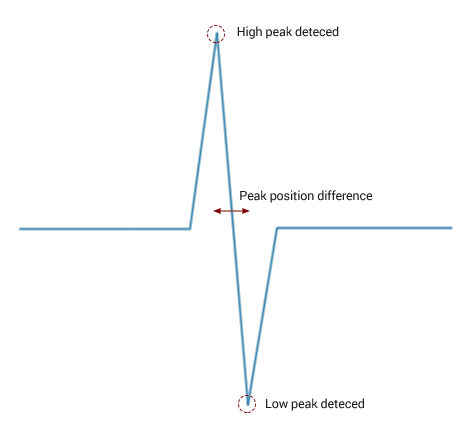
\includegraphics[width = 300 pt]{Img/Figures.png}
\caption{Block diagram}
\label{fig:BlockDiagram}
\end{figure}

\begin{equation}
\frac{n!}{k!(n-k)!} = \binom{n}{k}
\label{eq: myequation}
\end{equation}

Reference to equation \autoref{eq: myequation}.

\subsection{Sub section heading}
\lipsum[1-2]

\subsection{Sub section heading}
\lipsum[1-2]